\documentclass{IEEEtran}
\usepackage{mathtools}
\usepackage{graphicx}
\usepackage{amssymb}
\usepackage{amsmath}
\usepackage{pythonhighlight}
\usepackage[utf8]{inputenc}
\usepackage{fancyhdr}
\usepackage{pythonhighlight}
\usepackage{changepage}
\usepackage{slashbox}
\usepackage{floatrow}
\usepackage{listings}
\usepackage{derivative}
\usepackage[hidelinks]{hyperref}
\usepackage{fontawesome}
\usepackage{caption}
\usepackage{subcaption}
\usepackage[sorting=none,style=ieee]{biblatex}
\usepackage{cleveref}
\usepackage{algorithm}
\usepackage{algpseudocode}
\usepackage{physics}
\usepackage{lipsum}

\addbibresource{report.bib}
\title{Hodgkin and Huxley Cell Membrane Model Simulation}
\author{Kutay Ugurlu}

\begin{document}
\maketitle
\begin{abstract}
    The electrical behaviors of specific kinds of organs and structures in the human body provide crucial information about the workings of physiological-level structures and mechanisms of certain diseases. For diagnosis regarding such structures, many imaging methods have been developed exploiting these behaviors. To do so, a good understanding of electrical cell behavior is required. This report provides a theoretical background for the action potential behavior, using Hodgkin-Huxley's explanation, and explains the methodology to create a simulation software that illustrates the generation and propagation of the action potentials. The developed code is available online at \href{https://github.com/kutay-ugurlu/Hodgkin-Huxley-Membrane-Model}{https://github.com/kutay-ugurlu/Hodgkin-Huxley-Membrane-Model}
\end{abstract}
\section{Intro}
Hodgkin and Huxley \cite{hodgkin1952quantitative} published a series of five papers in 1952 to explain the generation mechanism of the action potential by introducing their experimental setup and the method. The first paper focused on explaining how neuron cells work. The second paper investigated the relationship between sodium ion concentration and the membrane voltage, also mentioning the action potential behavior. The third paper examined the effect of sudden conductance changes in the generation of the action potential. It was the fourth paper where Hodgkin and Huxley first explained the sodium inactivation phenomenon. In the last paper, the authors compiled their experimental results and came up with a formulation that explains the action potential generation process. 

\subsection{Voltage Clamp Experiment}

\begin{figure}[h]
\centering
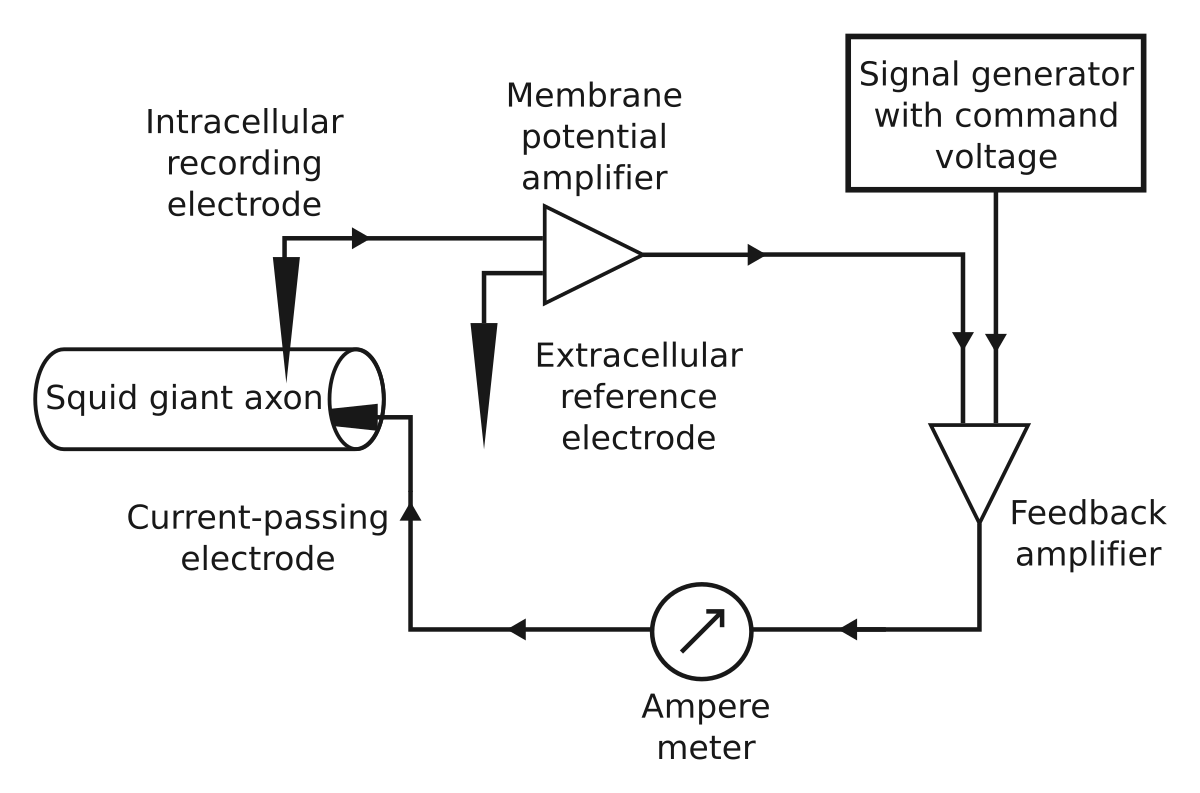
\includegraphics[width=\textwidth]{VCE.png}
\caption{Voltage Clamp Experiment Setup}\label{fig:vce}
\end{figure}

A voltage clamp is an experimental setup to measure the ionic currents that produce the electrical behavior of the excitable cells. It utilizes an iterative feedback mechanism, and the corresponding circuit, to achieve the desired or set voltage level of the membrane potential. Keeping the equivalent circuit model \Cref{fig:eqcct} and the equations governing the node voltage relations in this circuit, the researchers clamped the voltage at the Nernst potential and observed the transient and steady-state behavior of the resultant ionic currents. The measurement provided by these experiments paved the way to discovering the analytical relationship between cell membrane voltage and ionic conductances via curve fitting. 

\section{Theory}

\subsection{Mathematical Model}
\subsubsection*{Conductance}
The instantaneous conductances of different ion channels are calculated using the following relations:

\begin{align}
    g_{Na} &= m^3h \overline{g_{Na}} \label{eq:g1}\\
    g_{K} &= n^4 \overline{g_K} \label{eq:g2}\\
    g_{L} &= \overline{g_{L}}\label{eq:g3}
\end{align}

The parameters that control the change of conductances in terms of deviation from membrane voltage, \textit{i.e.} negative depolarization $V_{rest} - V_m$, are also expressed in first-order linear differential equations of time as follows:

\begin{align}
    \pdv{n}{t} &= \alpha_n(V_m)(1-n) - \beta_n(V_m)n \label{eqn:pdv1}\\
    \pdv{m}{t} &= \alpha_m(V_m)(1-n) - \beta_m(V_m)n \label{eqn:pdv2}\\
    \pdv{h}{t} &= \alpha_h(V_m)(1-n) - \beta_h(V_m)n \label{eqn:pdv3}
\end{align}

where $V_m$ is the deviation. \\

\subsubsection*{Activation and Inactivation Parameters}
The activation and inactivation parameters given in \Cref{eqn:pdv1,eqn:pdv2,eqn:pdv3} are formulated via curve fitting in Hodgkin and Huxley experiments. The resultans formulation are provided in \Cref{eqn:a1,eqn:a2,eqn:a3,eqn:b1,eqn:b2,eqn:b3}.

\begin{align}
    \alpha_n(V_m) &= \frac{0.01(10-V_m)}{e^{(1-0.1V)}-1} \label{eqn:a1}\\
    \alpha_m(V_m) &= \frac{0.01(25-V_m)}{e^{(2.5-0.1V)}-1} \label{eqn:a2}\\
    \alpha_h(V_m) &= 0.07e^{(\frac{-V}{20})} \label{eqn:a3}\\
    \beta_n(V_m) &= 0.125e^{(\frac{-V}{80})} \label{eqn:b1}\\
    \beta_m(V_m) &= 4e^{(\frac{-V}{18})} \label{eqn:b2}\\
    \beta_h(V_m) &= \frac{1}{e^{(3-0.1V)}-1} \label{eqn:b3}
\end{align}
\\
\\

\subsubsection{Equivalent Circuit Model}
\begin{figure}[h]
\centering
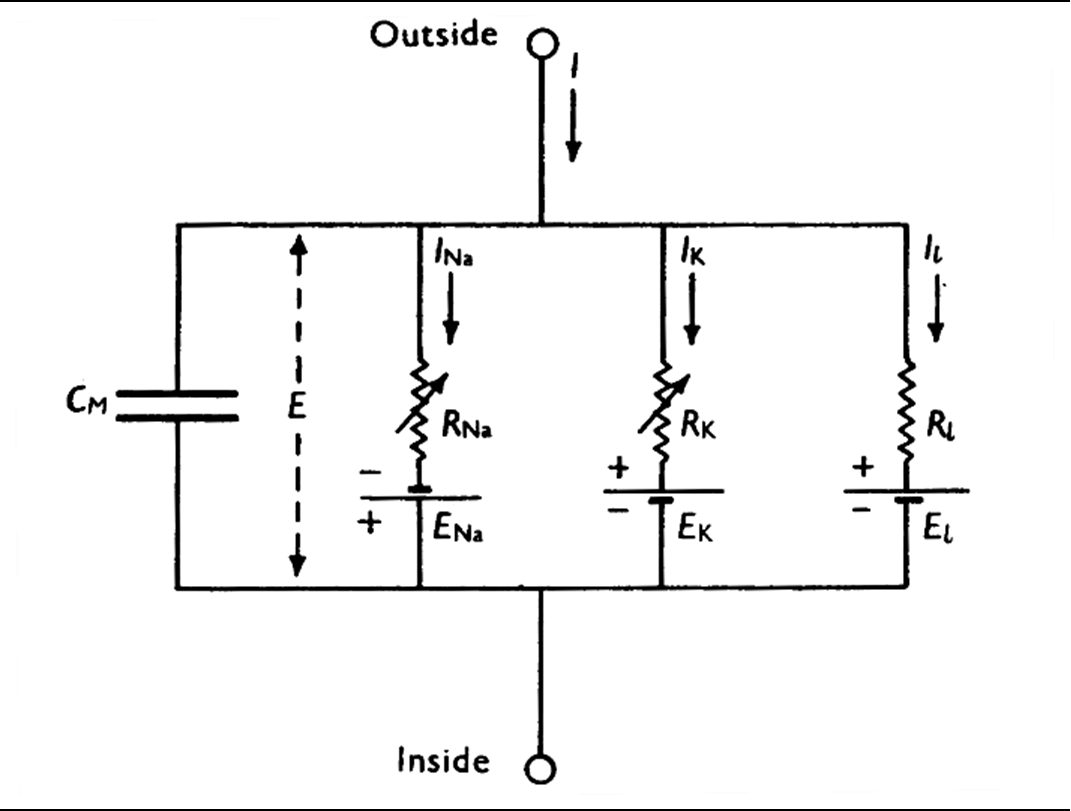
\includegraphics[width=0.8\textwidth]{EQCCT.png}
\caption{Equivalent Circuit of Hodgkin and Huxley membrane model}\label{fig:eqcct}
\end{figure}

Employing the node relations on the equivalent circuit, one can derive the relations given in \Cref{eqn:node1,eqn:node2,eqn:node3,eqn:kirch1,eqn:kirch2} for any time, hence any value of negative depolarization.

\begin{align}
    I_{Na} &= g_{Na}(V_{membrane} - \mathcal{E}_{Na}) \label{eqn:node1}\\
    I_{K} &= g_{K}(V_{membrane} - \mathcal{E}_{K}) \label{eqn:node2}\\
    I_{Cl} &= g_{L}(V_{membrane} - \mathcal{E}_{Cl}) \label{eqn:node3}\\
    I_{ionic} &= I_{Na} + I_{K} + I_{Cl} \label{eqn:kirch1}\\
    I_{Capacitive} &= I_{total} - I_{ionic} \label{eqn:kirch2}\\
    \Delta V_m &= I_{Capacitive}(i)dt / C_m; \label{eqn:cap}
\end{align}

where $I_{total}$ is the stimulation current applied to the cell. 

\subsubsection{Action Potential Propagation}

In addition to the time behavior of an action potential on a single point, the behavior of the action potential propagating on an axon is also important to have a complete understanding of the space-time behavior of the action potentials. To derive the formulation that explains such a concept, one needs to model the patch of a membrane.

\begin{figure}[h]
\centering
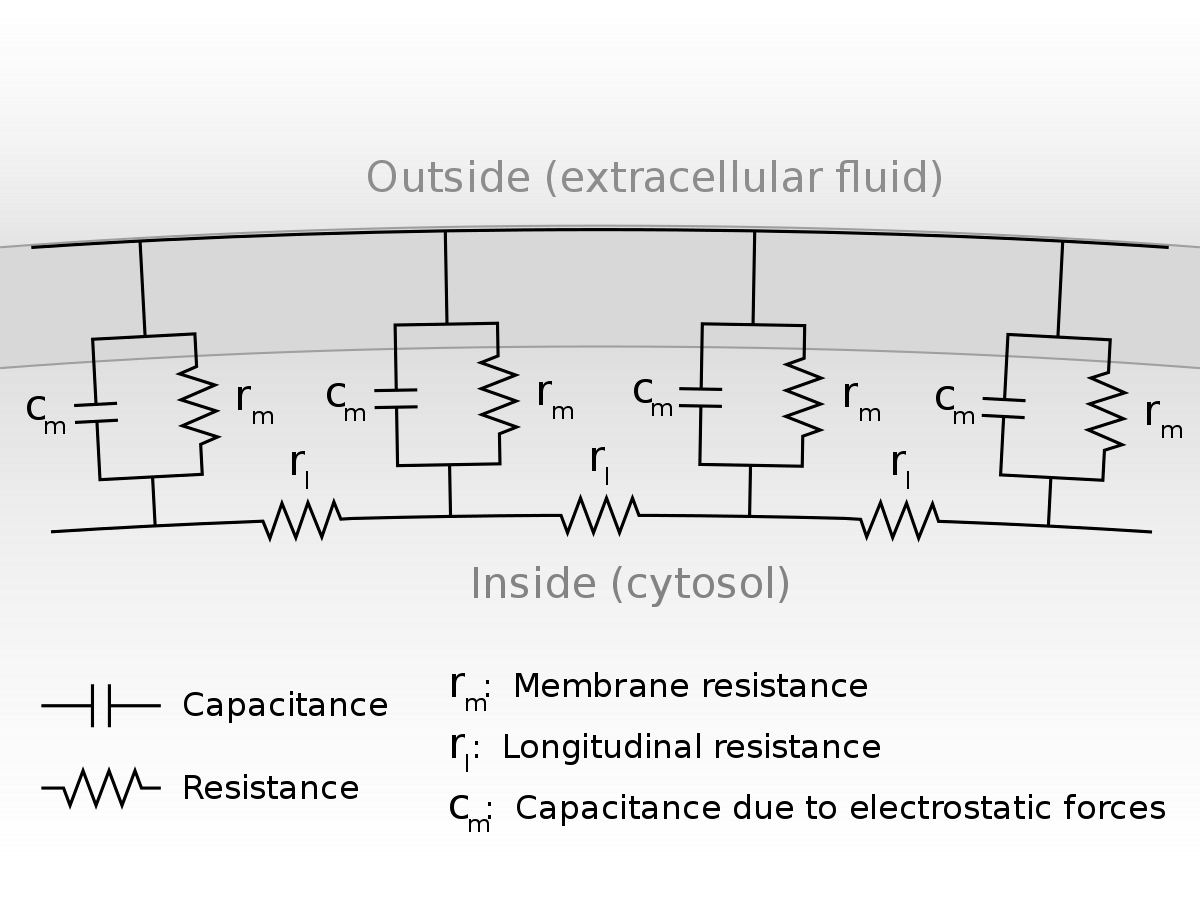
\includegraphics[width=0.8\textwidth]{1200px-Cable_theory_Neuron_RC_circuit_v3.svg.png}
\caption{Cable Model \cite{CableTheory}}\label{fig:approp}
\end{figure}

By using the model illustrated in \Cref{fig:approp}, \Cref*{eqn:cable} can be derived. 
\begin{equation}
    \pdv[2]{V_m}{x} = (r_i+r_e) i_m + r_i i_s \label{eqn:cable}
\end{equation}
where $i_m$ is the axial current defined from the extracellular region to the intracellular region and $i_s$ in the input stimulation current. 

Using the general cable equation defined in \Cref{eqn:cable}, \Cref{eqn:num} can be utilized to calculate the current along the entire axon given the stimulation current: 

\begin{equation}
    I_{total} = I_{stim} + \frac{\pdv[2]{V_m}{x} + r_eI_{stim}}{2\pi a (r_i+r_e)} \label{eqn:num} 
\end{equation}

In the numerical implementation, however, the second-degree partial derivative term should be replaced with its numerical approximation: 

\begin{equation}
    \pdv[2]{V_m}{x} = \frac{(V(x-1)-V(x))-(V(x)-V(x+1))}{\Delta x^2}
    \label{eqn:current}
\end{equation}

\subsection{Method}

\subsubsection{Implementation Environment}
The software is developed in MATLAB R2022(The MathWorks, Inc., Natick, Massachusetts, United States) along with the graphical user interface. The user interface provides visualizations for selected state vectors along time and space depending on the simulation type. The pseudocode for the software developed is presented in \Cref{alg:apgen,alg:approp}. The screenshots of the graphical user interfaces along with the default inputs that result in outputs that illustrate the main features are presented in \Cref{fig:gui1,fig:gui2}.


\clearpage

\onecolumn{

\begin{figure}[h]
    \centering
    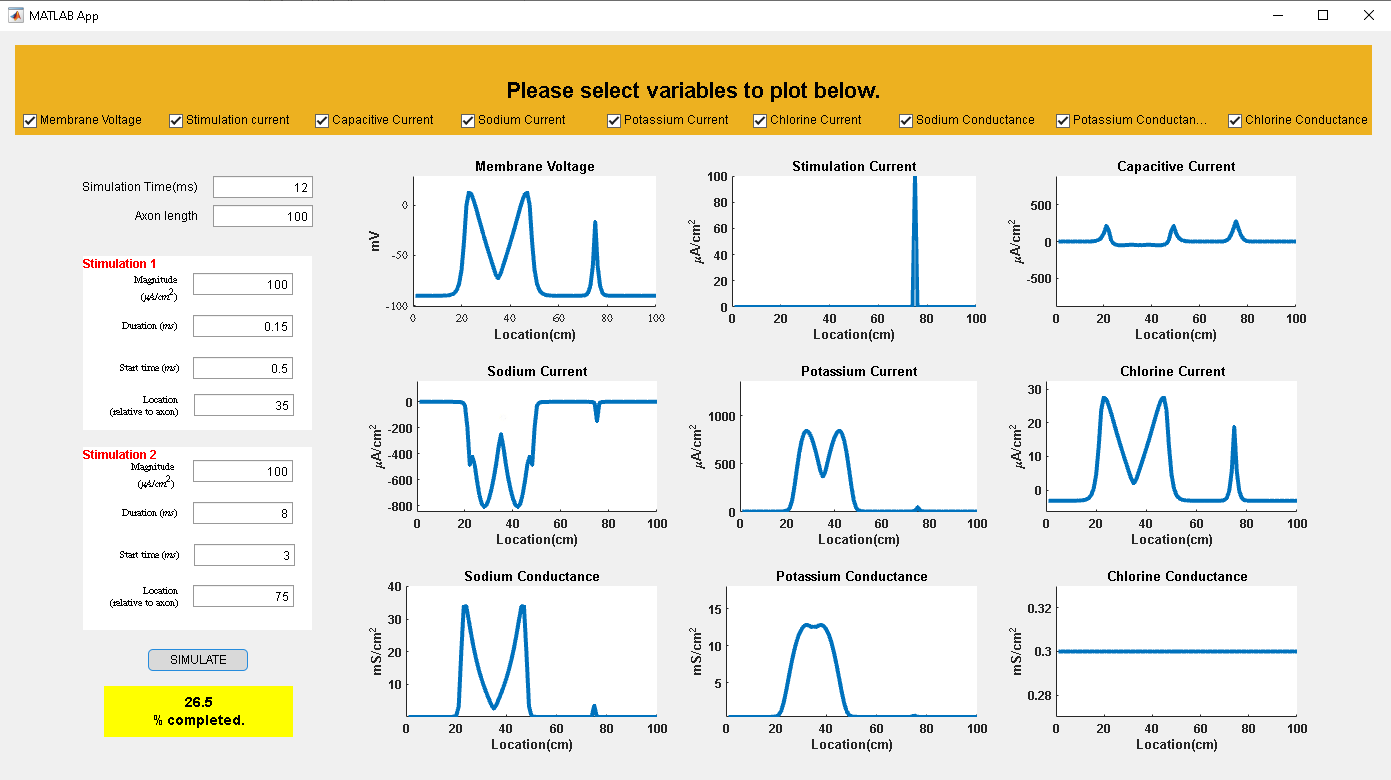
\includegraphics[width=0.8\textwidth]{GUI1.png}
    \caption{Action potential propagation software GUI}\label{fig:gui2}
    \end{figure}

    \begin{figure}[h]
        \centering
        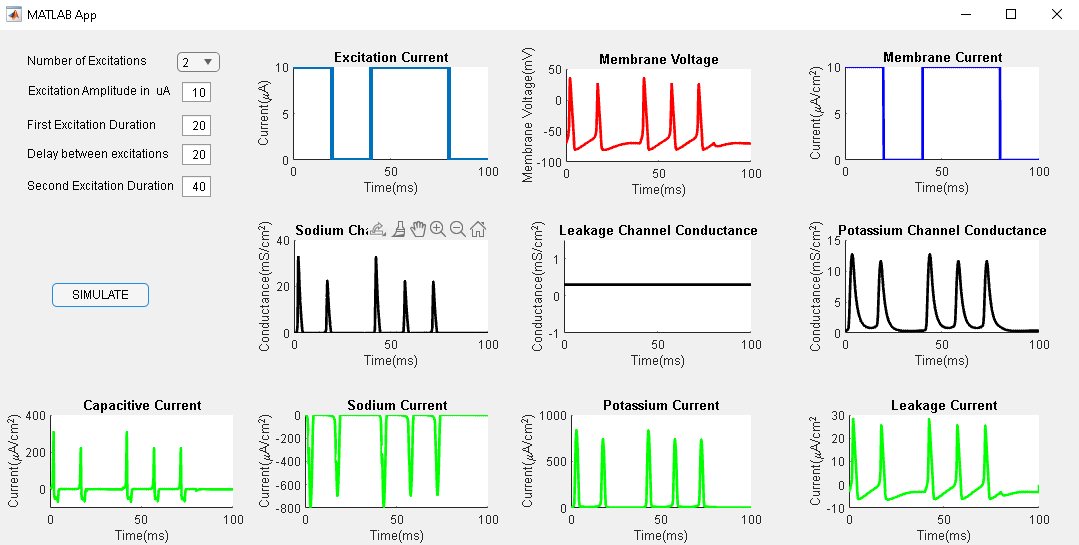
\includegraphics[width=0.8\textwidth, height=0.3\pdfpageheight]{GUI2.png}
        \caption{Action potential generation software GUI}\label{fig:gui1}
        \end{figure}
}

\twocolumn

\subsubsection{Generation}

For the generation part of the algorithm, the time steps are discretized and the update equations are constructed utilizing the differential \Cref{eqn:pdv1,eqn:pdv2,eqn:pdv3,eqn:cap}.

\begin{algorithm}[h]
    \caption{Action Potential Generation}\label{alg:apgen}
    \hspace*{\algorithmicindent}\textbf{Input}:\texttt{\#}Stim,Duration,Amplitude\newline
    \hspace*{\algorithmicindent}\textbf{Output}:Voltage, Current, Conductance
    \begin{algorithmic}[1]
    \Procedure{hhiterate}{${V_m}^{i}$} \label{proc:hhiterate}
        \State Calculate membrane voltage \Comment{$V_m = v_m + \Delta v_m$}. 
        \State Calculate $g(V_m)$ \Comment{\cref{eq:g1,eq:g2,eq:g3}}
        \State Calculate ionic currents. \Comment{\cref{eqn:node1,eqn:node2,eqn:node3}}
        \State Calculate capacitive current. \Comment{\cref{eqn:kirch1,eqn:kirch2}}
        \State Update $\Delta V_m$ \Comment{\cref{eqn:cap}}.
        \State Update m,n \& h. \Comment{\cref{eqn:pdv1,eqn:pdv2,eqn:pdv3}}
        \State \textbf{return} ${V_m}^{i+1}$
    \EndProcedure \\
    
    \Ensure $t_{stimulation} \le t_{simulation}$
    \State Assign cell parameters. \Comment{$C_m, \overline{g}_{Na,K,Cl}, \mathcal{E}_{Na,K,Cl}$}
    \State Initialize state vectors. \Comment{$G,m,n,h$}
    \State Assign initial values using $\alpha(0),\beta(0)$ 
    \State Design stimulation vector. \Comment{Use $\Delta t$}
    \For{$i=1, i<=Iteration Steps$}
        \State ${V_m}^{i+1} =$ \Call{hhiterate}{${V_m}^{i}$}
    \EndFor
    \State \textbf{return} $V_m, g, I$
    \end{algorithmic}
\end{algorithm}

\subsubsection{Propagation}

The stimulus, conductance, and current vectors are now initialized in two dimensions, representing the time and 1-dimensional space that represents the axon axis. Using \Cref{eqn:current}, the current along the axis is calculated for every time step of the simulation, and for each location, the \texttt{HHiterate} procedure defined in \Cref{alg:apgen} is called for the voltage update. 


\begin{algorithm}[h]
    \caption{Action Potential Propagation}\label{alg:approp}
    \hspace*{\algorithmicindent}\textbf{Input}:\texttt{\#}Stim,Duration,Amplitude, Axon Length\newline
    \hspace*{\algorithmicindent}\textbf{Output}:Voltage, Current, Conductance
    \begin{algorithmic}[1]
    
    \Ensure $t_{stimulation} \le t_{simulation}$
    \State Assign cell parameters. \Comment{$C_m, \overline{g}_{Na,K,Cl}, \mathcal{E}_{Na,K,Cl}$}
    \State Initialize state vectors. \Comment{$G,m,n,h$}
    \State Assign initial values using $\alpha(0),\beta(0)$ 
    \State Design stimulation vector. \Comment{Use $\Delta t$}
    \For{$t$: simulation time step}
    \For{$x$: discretized locations along the axon}
        \State Calculate current using \Cref{eqn:current}
        \State Employ \texttt{HHiterate} in \Cref{alg:apgen}
    \EndFor
    \EndFor
    \State \textbf{return} $V_m, g, I$
    \end{algorithmic}
\end{algorithm}

To guarantee convergence, the mesh ratio defined in \Cref{eqn:mesh} should be as small as possible:

\begin{equation}
    mesh ratio = \frac{\Delta t}{r_i c_m \Delta x^2} \label{eqn:mesh}
\end{equation}

\subsection{Results}

In this section, some characteristic behaviors of the action potentials during their generation and propagations are replicated through the developed software and the corresponding visualizations are going to be presented to illustrate and explain the associated mechanisms.

\begin{figure}[h]
\centering
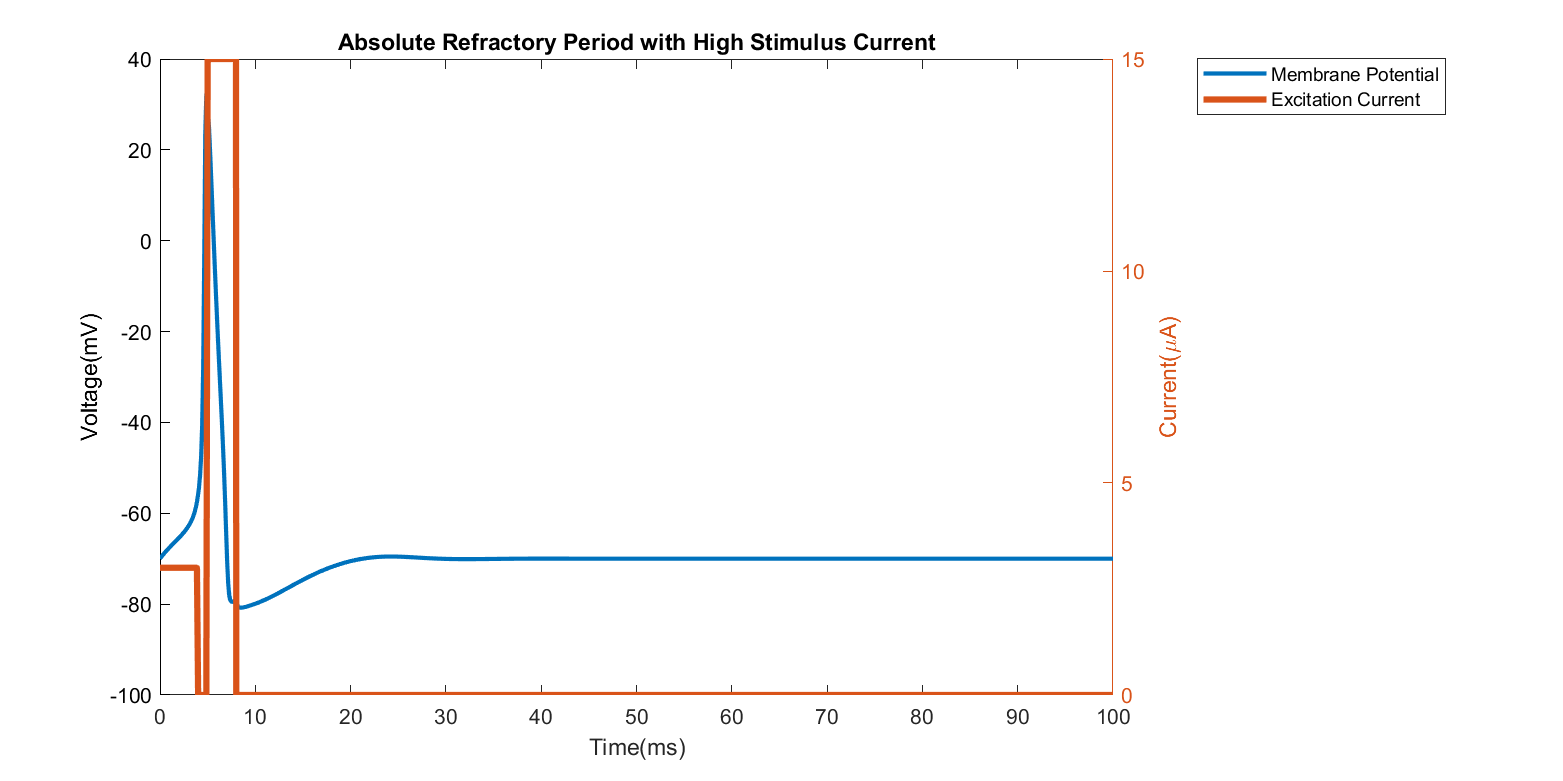
\includegraphics[width=\textwidth]{Fig5.png}
\caption{Absolute refractory period}\label{fig:arp}
\end{figure}
\begin{figure}[h]
\centering
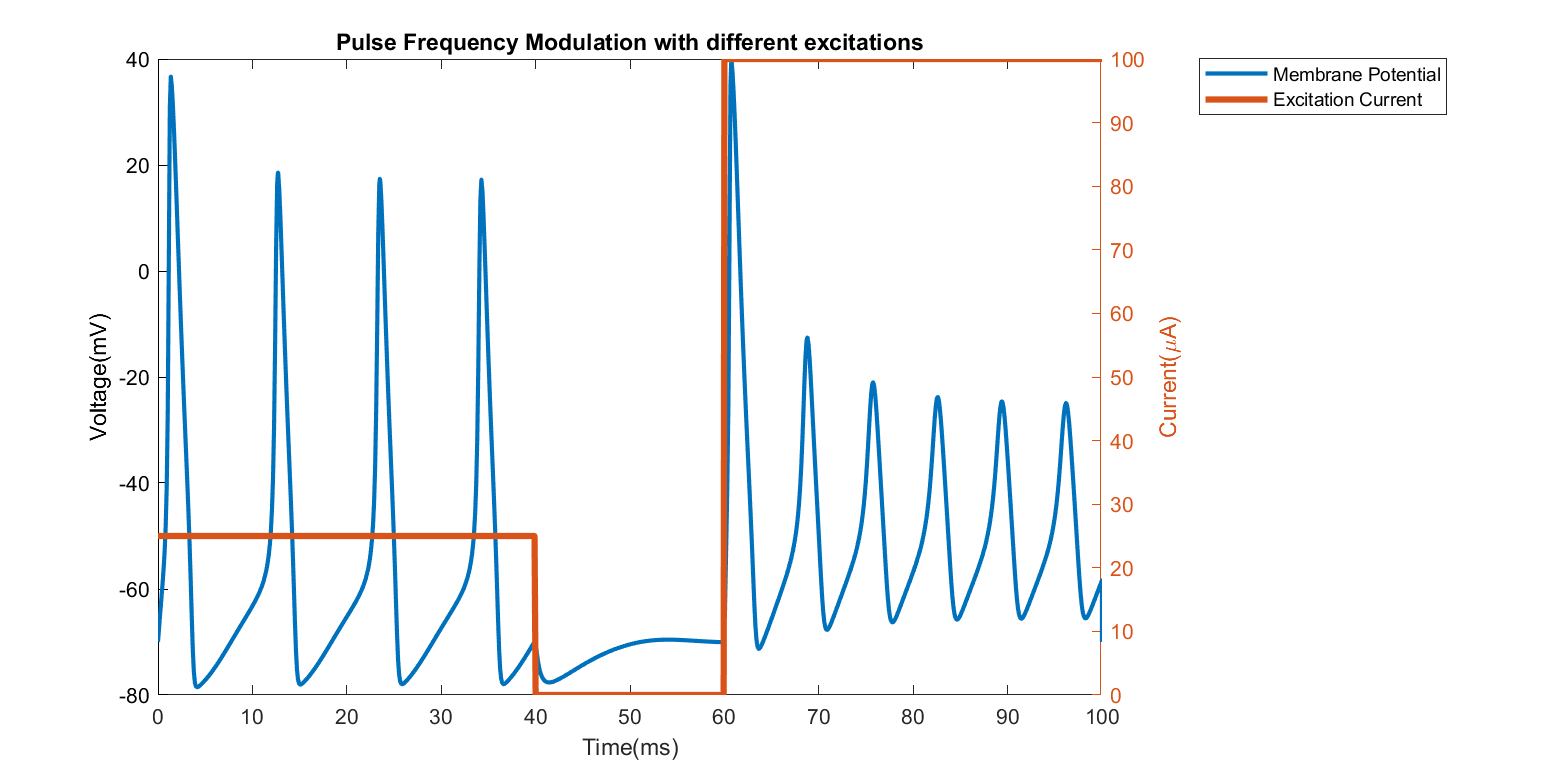
\includegraphics[width=\textwidth]{Fig2.png}
\caption{Frequency modulation}\label{fig:fm}
\end{figure}
\begin{figure}[h]
\centering
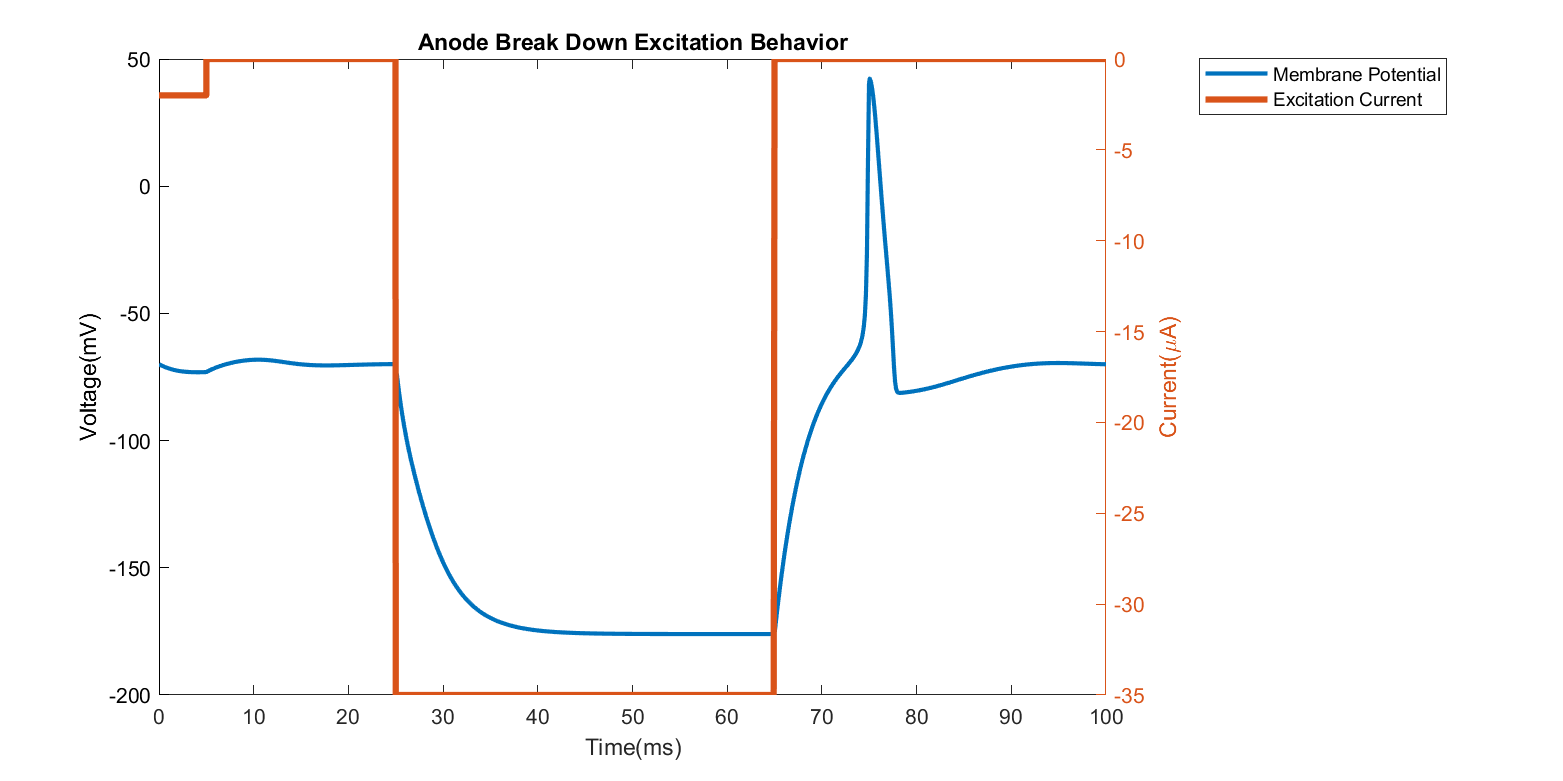
\includegraphics[width=\textwidth]{Fig4.png}
\caption{Anode breakdown excitation}\label{fig:abe}
\end{figure}
\begin{figure*}[h]
\centering
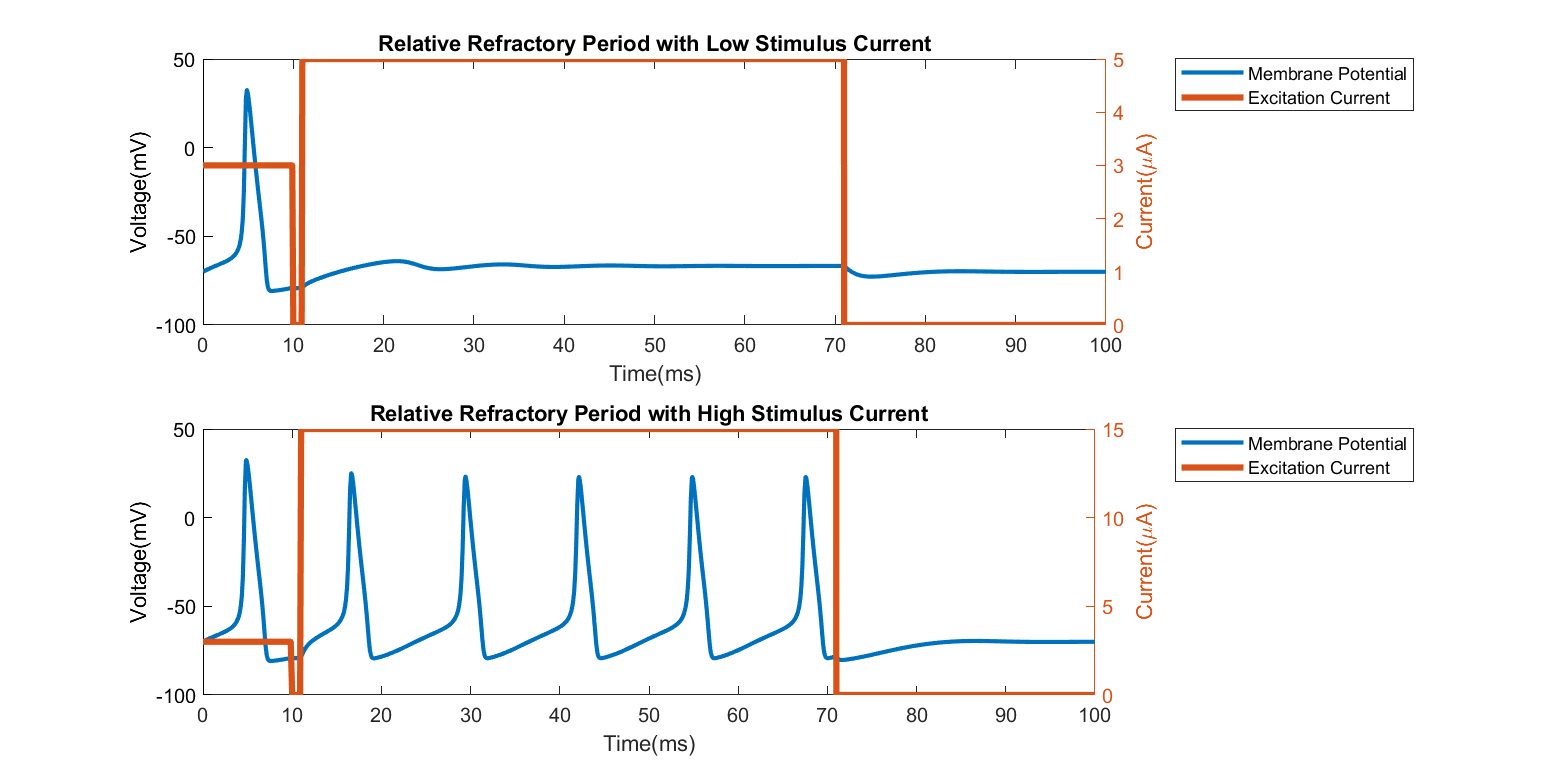
\includegraphics[width=\textwidth]{Fig6.png}
\caption{Relative refractory period}\label{fig:rrp}
\end{figure*}
\begin{figure}[h]
\centering
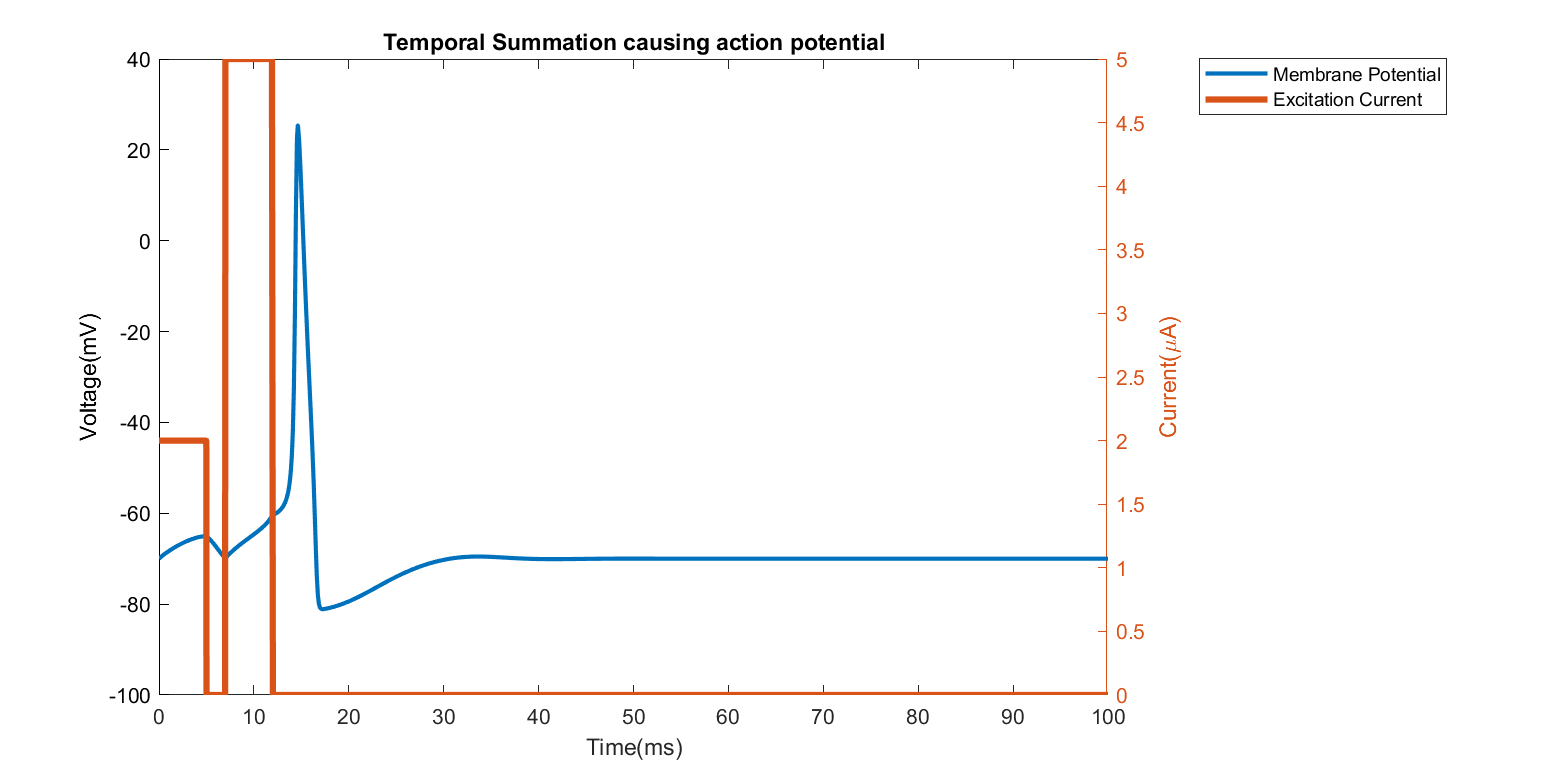
\includegraphics[width=\textwidth]{Fig1.png}
\caption{Temporal summation}\label{fig:tempsum}
\end{figure}
\begin{figure}[h]
\centering
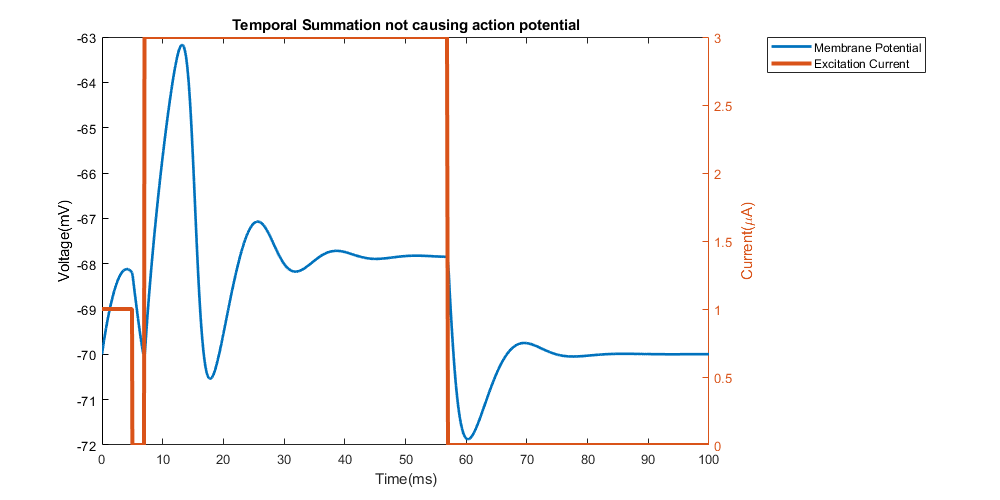
\includegraphics[width=\textwidth]{ts_not.png}
\caption{Temporal summation under subthreshold condition}\label{fig:ts_not}
\end{figure}
\vfill\null\newpage %%%%%%%%%%%%%%%%%%%%%%%%%%%%%%%%%%
\begin{figure}[h]
\centering
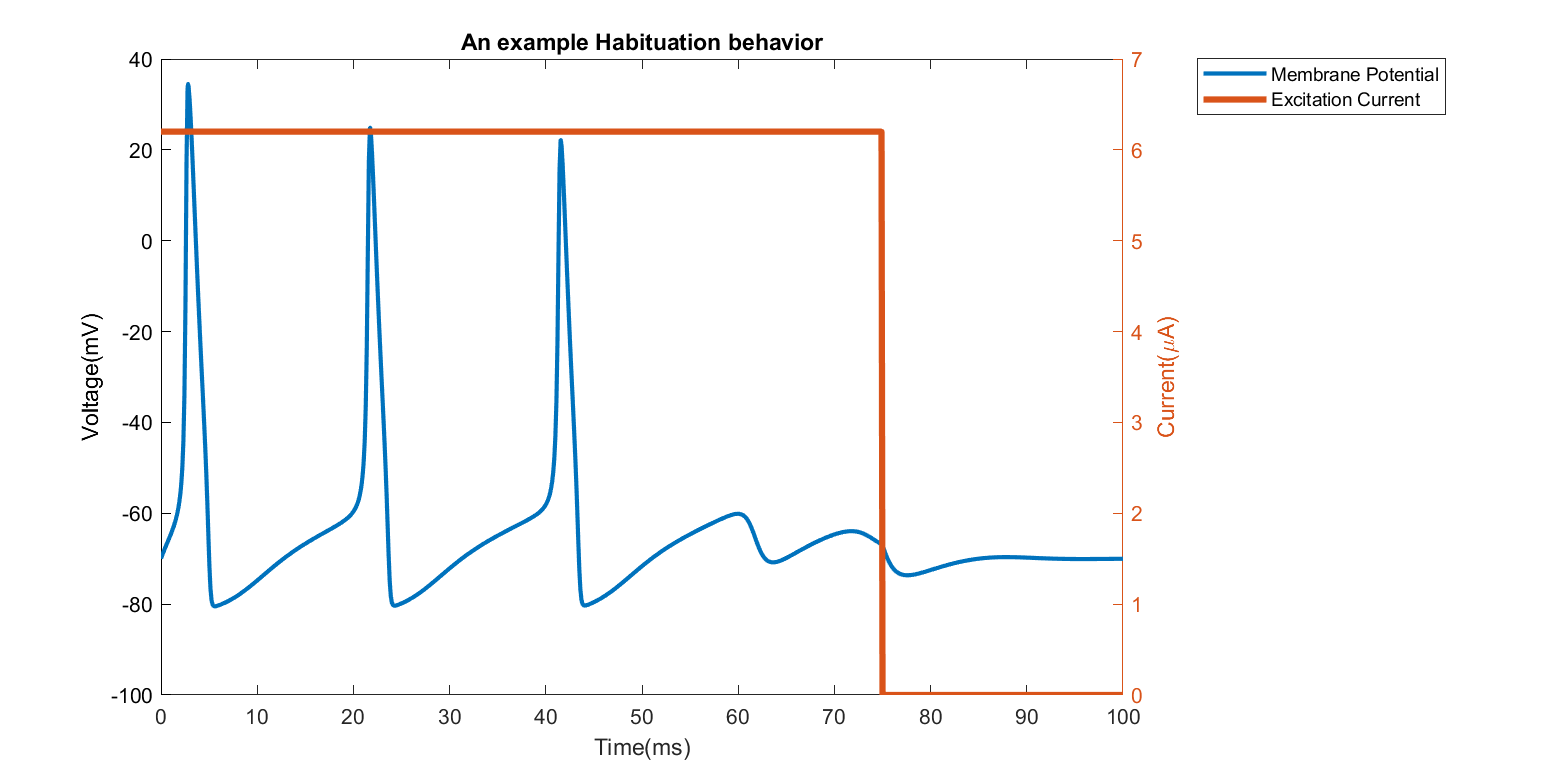
\includegraphics[width=\textwidth]{Fig3.png}
\caption{Habituation}\label{fig:habit}
\end{figure} 
\begin{figure}[h]
\centering
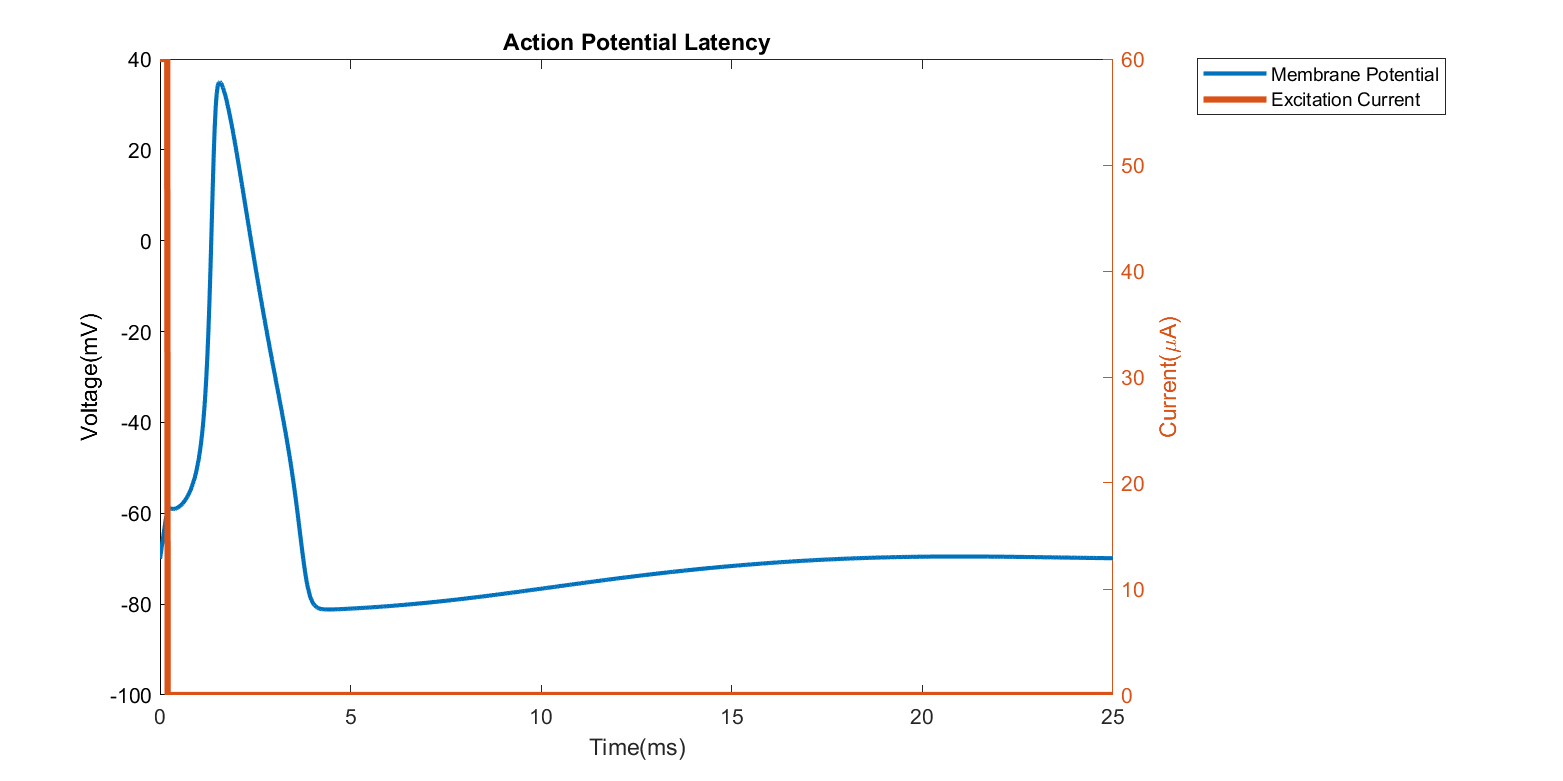
\includegraphics[width=\textwidth]{Fig7.png}
\caption{Action potential latency}\label{fig:apl}
\end{figure}
\vfill\null
\newpage %%%%%%%%%%%%%%%%%%%%%%%%%%%%%%%
\begin{figure*}[h]
\centering
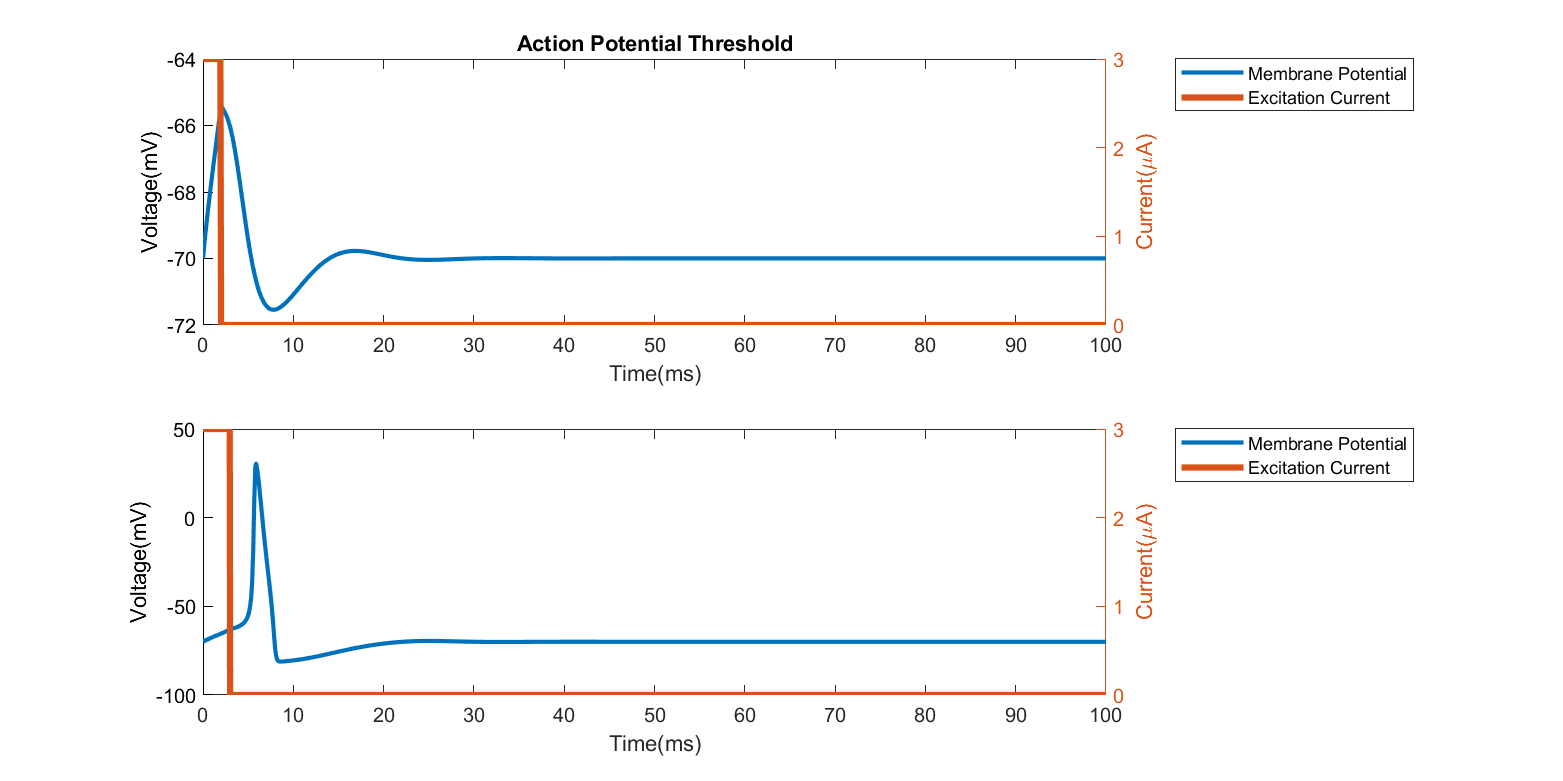
\includegraphics[width=\textwidth]{Fig8.png}
\caption{Action potential threshold}\label{fig:apth}
\end{figure*}
\begin{figure*}[h]
\centering
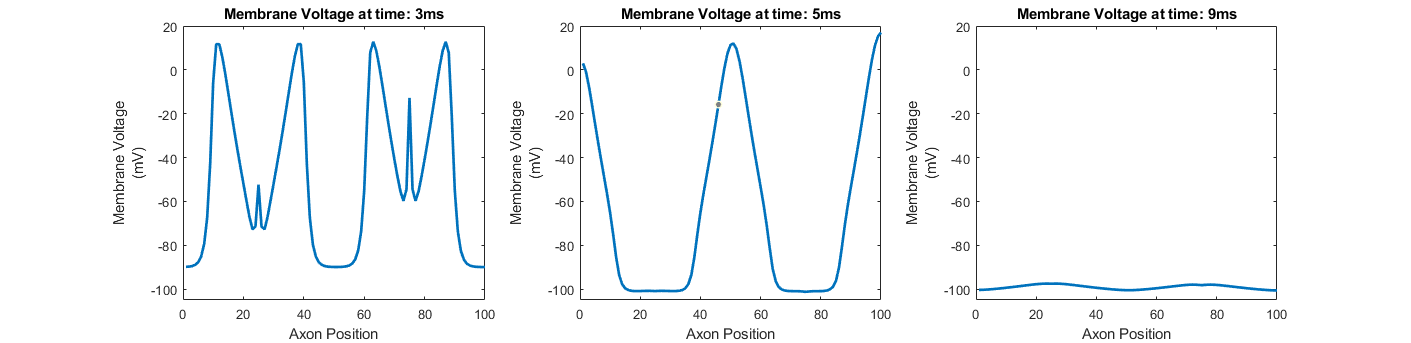
\includegraphics[width=\textwidth]{prop.png}
\caption{Propagation Behavior}\label{fig:propagation}
\end{figure*}
\vfill\null
\newpage %%%%%%%%%%%%%%%%%%%%%%%%%%%%%%%
\subsection{Discussion}
\subsubsection{Action potential threshold}
According to the Hodgkin Huxley model, the electrically active cells start to fire an action potential after the membrane voltage reaches a specific value called \textbf{Threshold voltage}. To investigate the value of the threshold voltage that is indirectly defined by the ionic concentrations of the cell, a series of software experiments are done. In \Cref{fig:apth}, one can observe that the cell did not fire an action potential for a membrane voltage of -66mV. In the subfigure at the bottom, however, we observe that there is a sharp increase in the membrane potential starting from around -65mV. Hence, it can be deduced that the threshold voltage is around -65 mV. It is important to note that the action potential generation does not stop even if the stimulus source is cut. 
\subsubsection{Absolute refractory period}
The absolute refractory period is defined as the time period after the repolarization when the cell cannot be excited again even with an abnormally high stimulus current. In \Cref{fig:arp}, we apply a 3$\frac{\mu A}{cm^2}$ stimulus for 5 milliseconds and observe that the action potential was fired. Shortly after that, in the repolarization phase of the cell, we again apply a stimulus, this time 5 times the magnitude of the first tone that started the action potential. However, at this time we observe that the cell did not fire an action potential. Hence, this region is in the absolute refractory period.
\subsubsection{Frequency Modulation}
Frequency modulation behavior is defined as a higher number of action potentials with a response to a higher stimulus at the same time period. In \Cref{fig:fm}, we see that two stimuli with amplitudes 25 and 100$\frac{\mu A}{cm^2}$ are applied to the cell for 40 ms. The higher stimulus resulted in 6 action potentials whereas the lower stimulus caused the cell to fire only 4 action potentials. With a 4 times higher stimulus, the frequency of action potential generation increased by 50\%. 
\subsubsection{Anode Breakdown Excitation}
Anode breakdown excitation describes the action potential generation behavior when the cell returns back to its resting state after being excited with a negative stimulation for a time period. In \Cref{fig:abe}, it can be observed that the cell is excited with -2$\frac{\mu A}{cm^2}$ stimulus for 3 milliseconds, and the membrane voltage went a little lower than the resting potential. when -35$\frac{\mu A}{cm^2}$ was applied to the cell for 40 milliseconds, the membrane behaved like an RC circuit under subthreshold conditions and the membrane voltage asymptotically approached approximately -180mV. When the stimulus is cut, the membrane voltage quickly returns to its resting value, however, it overshoots the threshold voltage while doing so. Hence, we observe an action potential generation after the membrane voltage reaches the threshold voltage. 
\subsubsection{Relative refractory period}
If a cell is stimulated with an \textbf{abnormally high} stimulus in the relative refractory period after the repolarization phase, the cell generates an action potential, although it does not respond to lower stimuli at the same phase. \Cref{fig:rrp} provides insight about this behavior. At the top figure, the cell is stimulated with 3$\frac{\mu A}{cm^2}$ for 10 milliseconds and the cell fires an action potential. When the cell is stimulated with a stimulus with a magnitude of 5$\frac{\mu A}{cm^2}$ for almost 60 milliseconds, it does not generate any response to the low stimuli. When we examine the figure at the bottom, the cell is stimulated with 15$\frac{\mu A}{cm^2}$, an abnormally high stimulus, for again 60 milliseconds. As a result, we observe that 5 action potentials are generated by the cell in response to this stimulus during the time it is applied.
\subsubsection{Temporal Summation} 
\Cref{fig:tempsum,fig:ts_not} illustrate two different scenarios with two different stimuli. The magnitude of the second stimulus is higher than that of the first one in both scenarios. Although we observe an action potential in the first scenario with the stimulus magnitude of 5$\frac{\mu A}{cm^2}$ for 5 milliseconds, the same response was not observed in the second scenario where the second stimulus of magnitude 3$\frac{\mu A}{cm^2}$ is applied for 50 milliseconds. The membrane voltage fluctuated around -67.5mV, exhibiting a subthreshold membrane behavior.
\subsubsection{Habituation}
Habituation can be defined as the decreased or ceased response of a cell to a constant electrical stimulus \cite{cheever1994habituation}. This behavior can be observed in \Cref{fig:habit}. A stimulus that has a magnitude high enough to trigger an action potential is applied to the cell at 75 milliseconds. After the first 3 action potentials, the cell stopped generating new action potentials. 
\subsubsection{Action Potential Latency}
Action potential latency refers to the latency between the stimulus application time and the start of depolarization. In the experimental scenario described in \Cref{fig:apl}, a 60$\frac{\mu A}{cm^2}$is applied for 0.2 milliseconds at the beginning of the inspection interval, causing a sudden decrease in the membrane voltage, from resting potential to around -60mV. Although the stimulus is cut, the membrane continues to depolarize until the membrane voltage reaches the threshold voltage and the cell triggers an action potential. This approximately 2 milliseconds of latency is called the action potential latency. 
\subsubsection{Ioinc Channel Conductances}
\Cref{fig:gui1} shows that the change in potassium conductance spans a wider range of time when compared to sodium conductance. Before depolarization, we observe an increase in the sodium conductance, allowing the sodium ions to flow into the cell which can be also interpreted by inspecting the negative valued sodium current. Short after depolarization, the potassium conductance increases, and potassium ions start to flow out of the cell, causing depolarization, via the positive valued potassium current. When compared to the sodium and potassium currents, the leakage current which is mainly composed of chlorine ions, can be observed to be orders of magnitude smaller. 
\subsubsection{Propagation}
\Cref{fig:propagation} illustrates a scenario with the following simulation variables:
\begin{itemize}
    \item Simulation time: 10 milliseconds
    \item Stimulation 1 Magnitude: 100$\frac{\mu A}{cm^2}$
    \item Stimulation 2 Magnitude: 300$\frac{\mu A}{cm^2}$
    \item Stimulation Durations: 3 milliseconds
    \item Stimulation 1 Start: 0.1 milliseconds
    \item Stimulation 1 Start: 0.5 milliseconds
    \item Axon Length: 100 cm
    \item Stimulation 1 location: 25cm
    \item Stimulation 2 Location: 75 cm
\end{itemize}
The membrane voltage as a result of this simulation is plotted on the whole axon as snapshots taken at 3, 5, and 9 milliseconds after the beginning of the simulation. In the left figure, we observe that both of the stimuli have already triggered action potentials that are propagating through both directions. At the same time, at the location where the stimulus is applied, the membrane exhibits subthreshold behavior and the membrane voltage has the form of a symmetric decaying exponential $e^\frac{|z|}{\tau}$. In the middle figure, we realize that the stimulation is cut and we observe that the action potential waves that propagate through each other are "added". However, this behavior is not in the conventional wave constructive interference sense since we observe that the summed action potential has the same peak value as the individual components. In the figure on the right, \textit{i.e.} 4 milliseconds later than the previously illustrated case, we observe that the "outer" action potentials are diminished at the end of the axon, along with the summed action potential, which can be considered as a similar behavior of destructive interference.


\section{Future Work}
The formulation behind the developed software relies on some assumptions about the movement of ions in the cell. Given the computing power available today, these assumptions may be challenged and a more detailed ionic movement simulation can be conducted. The electrical properties of the cell membrane can be made variable to further analyze the spatial behavior of the action potential.

\section{Conclusion}
This project report constitutes the procedure of the development of software that exhibits and mimics the action potential generation behavior of an electrically active cell and action potential propagation on an axon. The characteristic behaviors of the action potential are realized through simulation and explained in terms of the simulation parameters. In addition, the behavior of propagating action potentials in different directions is illustrated and examined.

\printbibliography{}
\end{document}

